
%! program = pdflatex

\documentclass[12pt]{article}
\usepackage{amsmath}
\usepackage{natbib}
\usepackage{graphicx}
\usepackage{amssymb}
\usepackage{epstopdf}
\usepackage{float} % to keep the figures in place

\usepackage{caption}
\usepackage{subcaption}
\usepackage{color}
\usepackage{undertilde}
\usepackage{enumitem}
\newcommand{\cred}{ \color{red}}
\newcommand{\cgreen}{\color{green}}
\newcommand{\cblue}{\color{blue}}
\newcommand{\cmag}{\color{magenta}}
\newcommand{\bn}{\begin{enumerate}}
\newcommand{\en}{\end{enumerate}}
\newcommand{\bi}{\begin{itemize}}
\newcommand{\ei}{\end{itemize}}
\newcommand{\be}{\begin{eqnarray}}
\newcommand{\ee}{\end{eqnarray}}
\newcommand{\by}{\begin{eqnarray*}}
\newcommand{\ey}{\end{eqnarray*}}
\renewcommand{\labelenumi}{(\alph{enumi}) }
%
\usepackage[margin=2.2cm, includehead]{geometry}% see geometry.pdf on how to lay out the page. There's lots.
\geometry{letterpaper} % or letter or a5paper or ... etc
% \geometry{landscape} % rotated page geometry
%\bibpunct{(}{)}{;}{a}{,}{,}
%\setlength{\textwidth}{16cm}
%\setlength{\textheight}{21cm}
\def\nonumber{\global\@eqnswfalse}
\newcounter{parnum}
\newcommand{\N}{%
  \noindent\refstepcounter{parnum}%
   \makebox[\parindent][l]{\textbf{[\arabic{parnum}]}}\quad  }
% Use a generous paragraph indent so numbers can be fit inside the
% indentation space.
\setlength{\parindent}{1.5em}

% See the ``Article customise'' template for come common customisations

\date{}
%\date{} % delete this line to display the current date

%%% BEGIN DOCUMENT
\usepackage{Sweave}
\begin{document}
\Sconcordance{concordance:aagarwal.tex:aagarwal.Rnw:%
1 51 1 1 0 36 1 1 163 112 1}

%\large
%\maketitle
\newtheorem{thm}{Theorem}[section]
\newtheorem{cor}[thm]{Corollary}
\newtheorem{lem}[thm]{Lemma}
\newtheorem{prop}[thm]{Proposition}
\newtheorem{defn}[thm]{Definition}
\newtheorem{exam}[thm]{Example}
\newtheorem{qstn}[thm]{Question}

%%%
\newpage
\begin{center}
{\bf Final take-home exam - STAT 515}\\
Amal Agarwal
\end{center}
%==========================
\section*{Answer 1}
\begin{enumerate}[label=(\alph*)]
\item The target density $\pi(\beta_1|\utilde{Y},\utilde{X})$ upto a normalizing constant is given as:
\[\pi(\beta_1|\utilde{Y},\utilde{X})\propto \text{exp}\left(\lambda\beta_1\sum_{i=1}^{n}X_i-\dfrac{\beta_1^2}{200}\right)\prod_{i=1}^{n}\text{erfc}\left(\dfrac{\beta_0+\beta_1 X_i+\lambda\sigma_i^2-Y_i}{\sqrt{2}\sigma_i}\right)=h(\beta_1)\]

Random Walk Metropolis algorithm  was used to approximate the posterior distribution $\pi(\beta_1|\utilde{Y},\utilde{X})$ with the proposal being normally distributed as $N(\beta_1^{(t)},\tau^2)$. Here $\beta_1^{(t)}$ is the current state and $\tau^2$ is the tuning parameter. The corresponding pseudocode is given as follows:

\begin{itemize}
\item Start off with $\beta_1^{(0)}$ in the support $(-\infty,+\infty)$ chosen arbitrarily. Choose the sample size $m$.
\item Run loop from $t=0:(m-1)$
\begin{itemize}
\item Generate a candidate $\beta_1^{*}$ from N($\beta_1^{(t)},\tau^2$)
\item Accept $\beta_1^{*}$ as next state $\beta_1^{(t+1)}$ with the following acceptance probability $\alpha$, else assign the current state as next state.
\[\alpha(\beta_1^{*},\beta_1^{(t)})=\text{min}\left(1,\dfrac{h(\beta_1^{*})}{h(\beta_1^{(t)})}\right)\]
where $h$ is the target kernel defined above.
\end{itemize}
\end{itemize}
The algorithm was run $3$ times with starting values as $7$, $7.2$ and $6.6$ based on several preliminary MCMC runs. The tuning parameter $\tau^2$  was set as $2$ chosen by trial and error that results in an ESS greater than $5000$ for a sample size of $30,000$.

\item Poterior estimate of $\beta_1$ is \textbf{7.3353} and the corresponding MCMC standard error is \textbf{0.00422}

\item $95\%$ credible interval for $\beta_1$ is (\textbf{6.725,7.9357})

\item See Fig.1 (c)
\item Fig.1 (a) indicates that the $3$ chains with different starting values converge to the same value of the estimate approximately. Fig.1 (b) shows that MCMC standard errors decays exponentially with number of iterations. Fig.1 (c) suggests that the smoothed density approximation after $n/2$ and $n$ samples don't differ significantly. Fig.1 (d) shows the decreasing profile of autocorrelation with increasing lag. Further the effective sample size was obtained as \textbf{5063}. These heuristics suggest that the approximations are accurate and the algorithm works fine.

\begin{figure}[H]
\begin{centering}
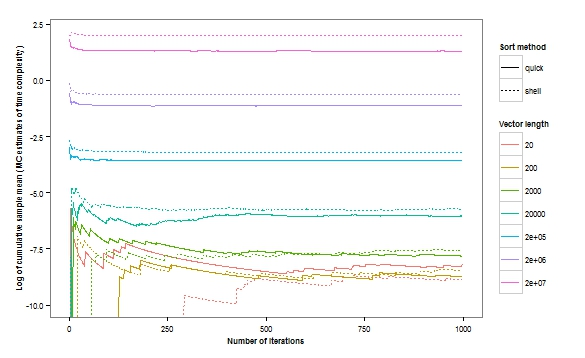
\includegraphics[scale=1.5]{fig1.jpeg}
\caption{(a) Poterior estimate of E($\beta_1$) vs. no. of iterations, (b) MCMC standard error E($\beta_1$) vs. no. of iterations, (c) Smoothed density plot of MCMC posterior samples and (d) Autocorrelation of samples vs. lag}
\end{centering}
\end{figure}
\end{enumerate}

\section*{Answer 2}
\begin{enumerate}[label=(\alph*)]
\item The target density $\pi(\beta_0,\beta_1,\lambda|\utilde{Y},\utilde{X})$ upto a normalizing constant is given as:
\[\pi(\beta_0,\beta_1,\lambda|\utilde{Y},\utilde{X})\propto \lambda^{n-0.99}\text{exp}\left[\dfrac{\lambda}{2}\sum_{i=1}^{n}\{2(\beta_0+\beta_1 X_i)+\lambda\sigma_i^2-2Y_i\}-\dfrac{\lambda}{100}\right]\prod_{i=1}^{n}\text{erfc}(z_i)\]
where $z_i=\dfrac{\beta_0+\beta_1 X_i+\lambda\sigma_i^2-Y_i}{\sqrt{2}\sigma_i}$
Variable one at a time Metropolis Hastings algorithm was used to approximate the above joint posterior distribution. The joint conditional of $\beta_0$ and $\beta_1$ and the full conditional of $\lambda$ were derived as:
\[\pi(\beta_0,\beta_1|\lambda,\utilde{Y},\utilde{X})\propto\text{exp}\left[\lambda\beta_0 n+\lambda\beta_1 \sum_{i=1}^{n}X_i\right]\prod_{i=1}^{n}\text{erfc}(z_i)=h_{\beta_0\beta_1}(\beta_0,\beta_1)\]
\[\pi(\lambda|\beta_0,\beta_1,\utilde{Y},\utilde{X})\propto\lambda^{n-0.99}\text{exp}\left[\dfrac{\lambda}{2}\sum_{i=1}^{n}\{2(\beta_0+\beta_1 X_i)+\lambda\sigma_i^2-2Y_i\}-\dfrac{\lambda}{100}\right]\prod_{i=1}^{n}\text{erfc}(z_i)=h_{\lambda}(\lambda)\]
where $z_i$ are defined as above.
The corresponding pseudocode is given as follows:
\begin{itemize}
\item Start off with $\beta_0^{(0)},\beta_1^{(0)},\lambda^{(0)}$ in the support $(-\infty,+\infty),(-\infty,+\infty),(0,+\infty)$ respectively. These starting values were chosen arbitrarily initially but later modified after several preliminary MCMC runs. Choose the sample size $m$.
\item Run loop from $t=0:(m-1)$
\begin{itemize}
\item Generate a candidate random vector $(\beta_0^{*},\beta_1^{*})$ from multivariate normal proposal N($(\beta_0^{(t)},\beta_1^{(t)}),\Sigma$). Here $\Sigma$ is a positive semi-definite matrix containing 3 independent tuning parameters. 
\item Random Metopolis update: Given the current state $\beta_0^{(t)},\beta_1^{(t)},\lambda^{(t)}$, accept $(\beta_0^{*},\beta_1^{*})$ as next state $(\beta_0^{(t+1)},\beta_1^{(t+1)})$ with the following acceptance probability $\alpha_{\beta_0\beta_1}$, else assign the current state $(\beta_0^{(t)},\beta_1^{(t)})$  as next state $(\beta_0^{(t+1)},\beta_1^{(t+1)})$.
\[\alpha_{\beta_0\beta_1}(\beta_0^{*},\beta_1^{*},\beta_0^{(t)},\beta_1^{(t)})=\text{min}\left(1,\dfrac{h_{\beta_0\beta_1}(\beta_0^{*}\beta_1^{*})}{h_{\beta_0\beta_1}(\beta_0^{(t)},\beta_1^{(t)})}\right)\]
\item Generate a candidate $\lambda^{*}$ from $\text{Gamma}(\text{scale}=\dfrac{(\lambda^{(t)})^2}{\tau_{\lambda}^2}$, \text{shape}=$\dfrac{\tau_{\lambda}^2}{\lambda^{(t)}})$
\item Metropolis hastings update (with proposal Gamma): Given the current state $\beta_0^{(t+1)},\beta_1^{(t+1)},\lambda^{(t)}$, accept $\lambda^{*}$ as next state $\lambda^{(t+1)}$ with the following acceptance probability $\alpha_{\lambda}$, else assign the current state $\lambda^{(t)}$  as next state $\lambda^{(t+1)}$.
\[\alpha_{\lambda}(\lambda^{*},\lambda^{(t)})=\text{min}\left(1,\dfrac{h_{\lambda}(\lambda^{*})\Gamma_{(\lambda^{*},\tau_{\lambda}^2)}(\lambda^{(t)})}{h_{\lambda}(\lambda^{(t)})\Gamma_{(\lambda^{(t)},\tau_{\lambda}^2)}(\lambda^{*})}\right)\]
where $h_{\beta_0,\beta_1}$, $h_{\lambda}$ are the target kernels as defined above and $\Gamma_{(\text{a},\text{b})}(\text{x})$ is the Gamma density evaluated at x with mean and variance as a and b respectively.
\end{itemize}
\end{itemize}
The above algorithm was run with starting vector $(\beta_0^{(0)},\beta_1^{(0)},\lambda^{(0)})$ as $(2.3,3.5,0.8)$ based on several preliminary MCMC runs. The tuning parameters were chosen as
\[\left(\Sigma=\begin{array}{ccc}
0.0187 & -0.0226 \\
-0.0226 & 0.0447 \\
\end{array} \right),\hspace{0.02in} \tau_{\lambda}^2=0.0036\]
by trial and error that results in the largest ESS possible for samples of $\beta_0, \beta_1$ and $\lambda$ along with satisfying other heuristics in part (d) for a sample size of $10,000$.

\item The following table gives the required information for a sample size of $10,000$:
\begin{table}[ht]
\centering
\begin{tabular}{rrrrr}
  \hline
Parameter & Posterior mean & MCMC standard error & $95\%$ credible interval \\ 
  \hline
$\beta_0$ & $2.33$ & $0.0053$ & $(2.05,2.61)$ \\ 
$\beta_1$ & $3.46$ & $0.0072$ & $(3.05,3.90)$ \\ 
$\lambda$ & $0.79$ & $0.0018$ & $(0.68,0.91)$ \\ 
   \hline
\end{tabular}
\end{table}

\item An approximation of the correlation between $\beta_0$, $\beta_1$ from the samples was computed as $-0.78$.

\item See Fig.3-Left panel.

\item The above algorithm was run for 3 chains with different starting values. Fig.2-left panel indicates that the $3$ chains with different starting vectors converge to the same value of the estimates approximately. Fig.2-Right panel shows that MCMC standard errors decays exponentially with number of iterations. Fig.3-Left panel suggests that the smoothed density approximation after $n/2$ and $n$ samples don't differ significantly. Fig.3-Right panel shows the decreasing profile of autocorrelation with increasing lag. Further the effective sample sizes were obtained as $(3575,4775,3280)$ for $(\beta_0,\beta_1,\lambda)$ respectively for a sample size of $50,000$. These heuristics suggest that the approximations are accurate and the algorithm works fine.
% \begin{figure}[H]
% \centering
%   \subcaptionbox{}{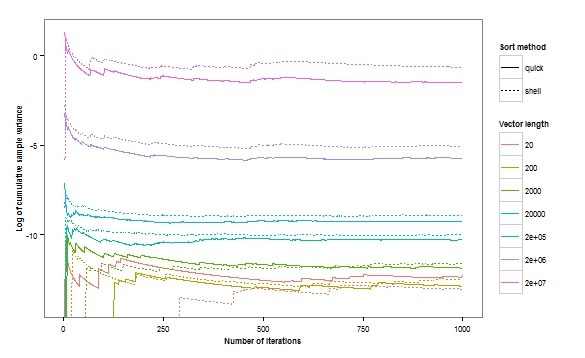
\includegraphics[width=3.1in]{fig2.jpeg}}\hspace{1em}%
%   \subcaptionbox{}{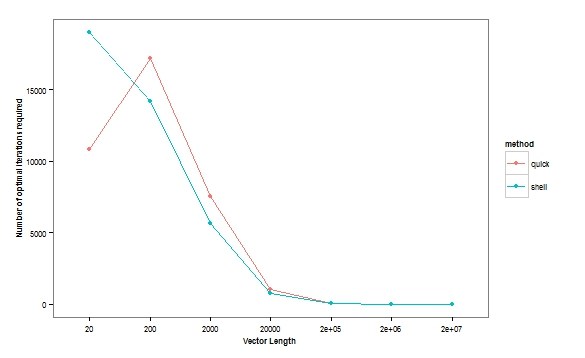
\includegraphics[width=3.1in]{fig3.jpeg}}
%   \caption{From top to bottom $\beta_0,\beta_1 $ and $\lambda$. (a)-left panel: Estimates of posterior means with number of iterations. (a)-right panel: MCMC standard errors with number of iterations. (b)-left panel: Smoothed density plots after sample sizes n/2 and n. (b)-right panel: Autocorrelation with lag.}
% \end{figure}
\begin{figure}[H]
\centering
  {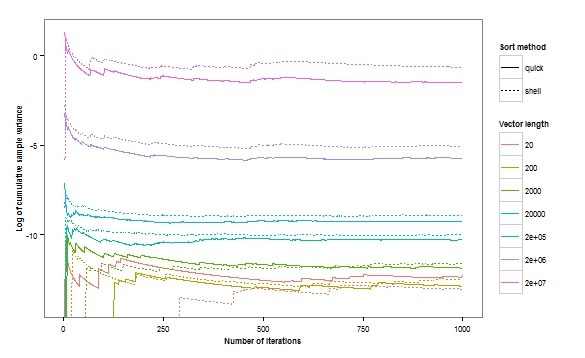
\includegraphics[width=4.5in]{fig2.jpeg}}
  \caption{From top to bottom $\beta_0,\beta_1 $ and $\lambda$. (a)-left panel: Estimates of posterior means with number of iterations. (a)-right panel: MCMC standard errors with number of iterations.}
\end{figure}
\begin{figure}
\centering
{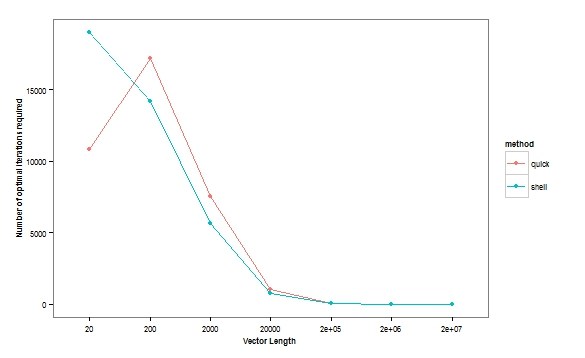
\includegraphics[width=3.9in]{fig3.jpeg}}
\caption{From top to bottom $\beta_0,\beta_1 $ and $\lambda$. Left panel: Smoothed density plots after sample sizes n/2 and n. Right panel: Autocorrelation of the samples vs. lag.}
\end{figure}

\end{enumerate}
\section*{Answer 3}
\begin{enumerate}[label=(\alph*)]
\item The following table gives the required information for a sample size of $10,000$:
\begin{table}[ht]
\centering
\begin{tabular}{rrrrr}
  \hline
Parameter & Posterior mean & MCMC standard error & $95\%$ credible interval \\ 
  \hline
$\beta_0$ & $0.1535$ & $0.0050$ & $(-0.1510,0.4652)$ \\ 
$\beta_1$ & $2.4629$ & $0.0081$ & $(1.9383,2.9928)$ \\ 
$\lambda$ & $0.1611$ & $0.0002$ & $(0.1509,0.1720)$ \\ 
   \hline
\end{tabular}
\end{table}
\item See Fig.4-left panel.
\begin{figure}[H]
\centering
  %\subcaptionbox{}{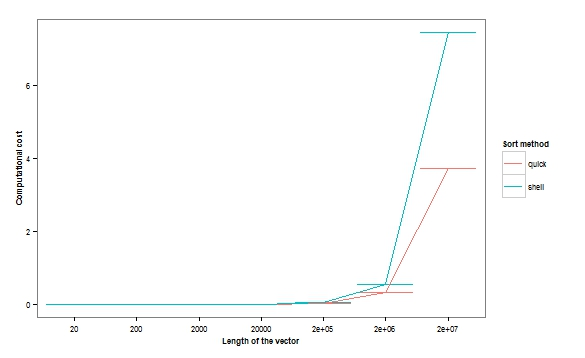
\includegraphics[width=3.1in]{fig4.jpeg}}\hspace{1em}%
  {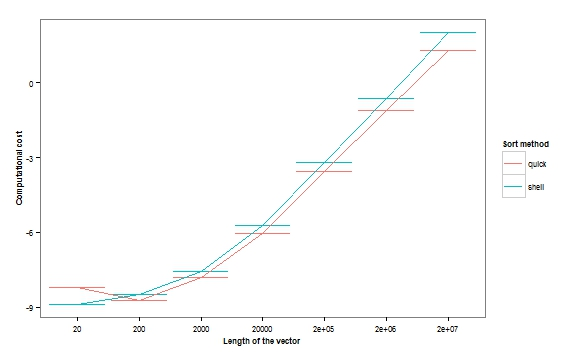
\includegraphics[width=4in]{fig5.jpeg}}
  \caption{From top to bottom $\beta_0,\beta_1 $ and $\lambda$. Left panel: Smoothed density plots after sample sizes n/2 and n. Right panel: Autocorrelation of the samples vs. lag.}
\end{figure}
\item MCMC algorithm was modified by tuning the parameters to the following values:
\[\Sigma=\left(\begin{array}{ccc}
0.0257 & -0.0371 \\
-0.0371 & 0.0765 \\
\end{array} \right),\hspace{0.02in} \tau_{\lambda}^2=2.9\times10^{-5}\]
The declining autocorrelations with lag, high ESS and other heuristics similar to Q2 suggests that the approximations are reliable in this case also.
\end{enumerate} 
\end{document}
